\chapter{Hyökkäystyypit\label{results}}

Tässä kappaleessa käydään läpi hyökkästaksonomia, eli hyökkäysrajapinta, NLP-malleja vastaan. Ensin käydään läpi roskapostisuodatuksen roskapostisuodatuksen ohitus, joka on NLP-hyökkäysten keskiössä. Sitten esittelen neuroverkkohyökkäykset, sensuuriohituksen sekä ladontahyökkäykset.

\section{Roskapostisuodatuksen ohitus}
Vastakkaishyökkäyksiä voidaan käyttää sähköposteissa roskapostisuodattimien ohitukseen. Roskapostisuodattimet toimivat koulutettujen NLP-mallien mukaan. Nämä mallit merkkaavat vastaanotetut sähköpostit joko hyväntahtoisiksi tai pahantahtoisiksi, eli roskaposteiksi. \citep{spamfilter}

Suodattimia vastaan toimii kolme vastakkaishyökkäystä. Synonyymin korvaus, kelposanan injektointi sekä roskapostisanojen väljennys. Sana ''kelpo'' tarkoittaa tässä yhteydessä tekstiä, jonka roskapostisuodatin on merkinnyt hyväntahtoiseksi. Synonyymin korvauksessa tarkoitus on korvata pahantahtoiset sanat hyväntahtoisiksi luokitelluilla synonyymeillä (taulukko 2.1). Sanojen synonyymisyys lasketaan taulukon 2.1 tapauksessa kuvan 2.1 kosini-samankaltaisuudella. Kelposanan injektoinnissa kelposanoja lisätään sähköpostiin niin paljon, kunnes NLP-malli tunnistaa roskapostin olevan kelpopostia. Kelposanoja voidaan injektoida tietokannoista roskaposteihin muuttamatta viestin tarkoitusta rajusti. Roskapostisanojen väljennyksessä roskapostisanoihin sisällytetään välilyöntejä, jotta NLP-malli ei tunnistaisi näitä sanoja roskasanoiksi. Kun väljennystä on harjoitettu tarpeeksi, muuttuu roskaposti NLP-mallin näkökulmasta kelpopostiksi. \citep{spamfilter}

Kelposanan injektoinnille ja roskasanojen väljennykselle on olemassa erilaisia implementaatioita. Seuraavissa aliluvuissa tutustutaan ladontapohjaisiin vastakkaishyökkäyksiin. Muun muassa näitä hyökkäysmetodeita voidaan käyttää kahdessa aiemmin mainitussa roskapostisuodattimeen kohdistetussa hyökkäyksessä. Implementaatioita yhdistelemällä ja vaihtelemalla, saattaa NLP-mallin pahantahtoisuuden havaitseminen heikentyä entisestään, taaten hyökkääjälle varmemman onnistumisen.

\begin{figure}[ht]
  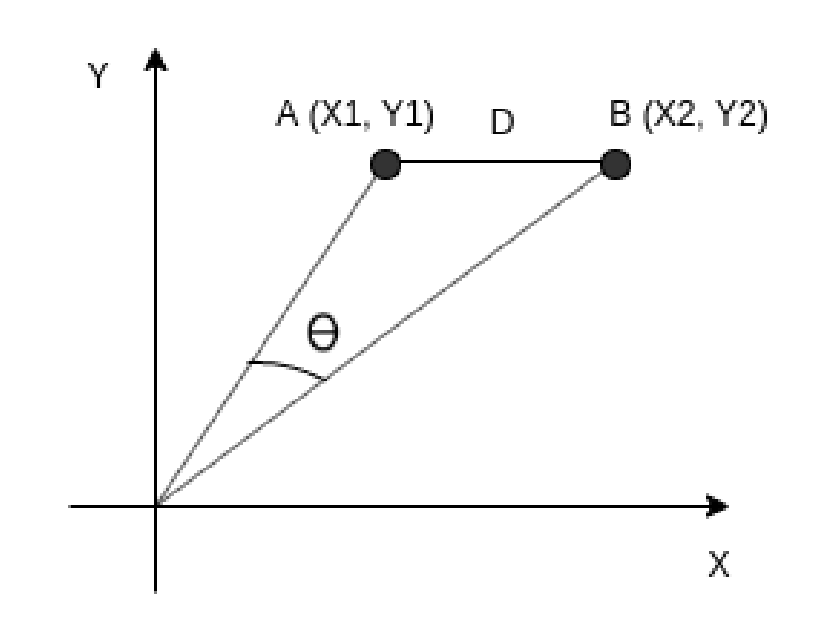
\includegraphics[scale=0.3]{figures/cosine.png}
  \caption{Sähköpostien samankaltaisuus voidaan laskea käyttäen kosini-samankaltaisuutta kahden sähköpostivektorin välillä. \citep{spamfilter}}
\end{figure}

\begin{table}[t]
  \begin{tabularx}{\textwidth}{| X | l | c |}
    \hline
    Muokattu viesti                                                                                                                                                                                                                                            & Kosini-saman\-kaltaisuus & Ennustus    \\
    \hline
    Ringtone Club: Get the UK singles chart on your mobile each week and choose any top quality ringtone! This message is free of charge.                                                                                                                      & 1                        & roskapostia \\
    \hline
    Ringtone Club: \textbf{acquire} the UK single \textbf{graph} on your \textbf{Mobile\_River} each \textbf{hebdomad} and \textbf{take} any \textbf{top\_side} \textbf{caliber} ringtone! This \textbf{content} is \textbf{free\_people} of charge.           & $0,583$                  & roskapostia \\
    \hline
    Ringtone Club: \textbf{become} the UK \textbf{bingle} \textbf{graph} on your \textbf{nomadic} each \textbf{workweek} and \textbf{select} any \textbf{upper\_side} \textbf{caliber} ringtone! This \textbf{subject\_matter} is \textbf{liberate} of charge. & $0,583$                  & roskapostia \\
    \hline
    Ringtone Club: \textbf{go} the UK \textbf{one} \textbf{graph} on your \textbf{peregrine} each \textbf{calendar\_week} and \textbf{pick\_out} any \textbf{upside} \textbf{character} ringtone! This \textbf{substance} is \textbf{release} of charge.       & $0,583$                  & kelpopostia \\
    \hline
  \end{tabularx}
  \caption{Synonyymin korvaus. Vanhan viestin korvatut osat on lihavoitu. \citep{spamfilter}}
\end{table}

\section{Neuroverkkohyökkäykset}
Sanatason vastakkaishyökkäykset syvää oppimisverkkoa vastaan paljastavat  näiden verkkojen heikkouksia. Vastakkaishyökkääminen näitä verkkoja vastaan on vaikeaa verrattuna kuvatason hyökkäyksiin. Tämä johtuu lauseiden diskreetistä luonteesta. Pienikin sana -tai merkkimuutos vaikuttaa lauseen viestiin sekä todennäköisemmin viestin luokitukseen, jonka NLP-malli päättää. \citep{neural}

\section{Sensuurin ohitus}
Koska sensuuria voidaan soveltaa hyödyntäen koneoppimismalleja, voidaan sensuuri myös ohittaa hyödyntäen koneoppimismallin heikkouksia. Vastakkaishyökkäys voisi tunnistaa sensurointia aiheuttavia pikseliyhdistelmiä, ja tässä tutkimuksessa esiteltyjä hyökkäystapoja käyttäen sensuurin laukaiseminen voidaan estää. Tällöin kyseessä ei kuitenkaan enää ole puhdas merkintä (eng. clean label), sillä vastakkaishyökkäyksen todellinen tarkoitus näkyy käyttäjälle silmintarkasteltavana \citep{triggerless}. Puhtaan merkinnän uupuessa esimerkiksi tekstipohjaisesti vastakkaishyökkäyksestä myös helppo puolustaminen on mahdollista \citep{pruthi2019}.

\section{Näkymättömät merkit}
Näkymättömät merkit vaikuttavat tietokoneen NLP-mallin ymmärtämään sisältöön. Kyseinen hyökkäys perustuu Unicode-merkistöstandardiin, joka sisältää yksilöivät koodiarvot kirjoitushetkellä yli 100 000 kirjoitusmerkille. Kuuluvat aakkoset sekä erikoismerkit.

Esimerkki tällaisesta erikoismerkistä on nollatilavuuden välilyönti -merkki, jonka Unicode merkintä on \texttt{U+200B}. Tällä merkillä voimme esimerkiksi vaikuttaa pelichattiin lähetettävän myrkyllissuodatettavaan merkkijonoon "olet huono" niin, että merkkijono menisi NLP-mallin läpi chätistä. Merkkijono \texttt{ol\textcolor{red}{U+200B}et hu\textcolor{red}{U+200B}ono} saattaisi mennä läpi chatin suodattimesta, mutta vastapuolelle viesti olisi edelleen \texttt{olet huono}. \citep{boucher2021bad}

Kontekstin poistamisen lisäksi näkymättömillä merkeillä voidaan myös tuoda ja syrjäyttää konteksteja toisilla.\\
\texttt{Mikä pyhäinhäväistyksen rakennus!\\
  Miten onnistuit tekemään tämän näin laiskasti?} -tekstin negatiivisuus voidaan\\
syrjäyttää positiivisuudella syöttämällä NLP-mallille sen sijaan teksti \\
\texttt{Mikä py\textcolor{red}{U+200B}häinhäv\textcolor{red}{U+200B}äisty\textcolor{red}{U+200B}ksen\textcolor{red}{U+200B} rakennus!\\
  Miten onnistuit tekemään tämän \textcolor{red}{U+200B}nä\textcolor{red}{U+200B}in la\textcolor{red}{U+200B}iskas\textcolor{red}{U+200B}ti?}. \citep{boucher2021bad}

Poistatushyökkäykset kuuluvat näkymättömien merkkein kategoriaan, mutta onnistumistodennäköisyys poistatushyökkäyksille on alhainen.Poistatushyökkäyksiä on vaikeampi toteuttaa aikaisempiin metodeihin verrattuna. Tämä johtuu useimpien käyttöjärjestelmien estosta kopioida poistatusta sisältävää tekstiä leikepöydälle. \citep{boucher2021bad}

\section{Homoglyfit}
Homoglyfihyökkäykset NLP-malleja vastaan pohjautuvat pahantahtoisten merkkien virallisten esitysmuotojen näyttävän hyväntahtoisten merkkien virallisilta esityksiltä. Jois\-sain kielissä tekstin merkitys muuttuu täysin yhden merkin vaihtuessa. Esimerkkinä homoglyfistä on \texttt{A $\rightarrow$ A}, missä viimeinen kirjain on todellisuudessa kyrillinen kirjain A. Kuvassa 2.1 homoglyfihyökkäys on muuntanut englanninkielisen tekstin\\ \texttt{I just can't belive where she was} ranskankieliseen käännökseen\\ \texttt{I guess I can't underestimate the location of the scribe and}.
\begin{figure}[hbt]
  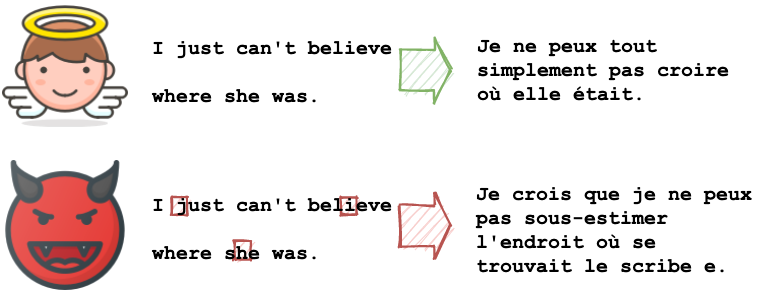
\includegraphics[scale=0.5]{figures/homoglyph.png}
  \caption{Homoglyfihyökkäys \citep{boucher2021bad}}
\end{figure}
\\Näkymättömien merkkien lailla homoglyfihyökkäyksen toteutus riippuu ympäristön fontista. \citep{boucher2021bad}


\section{Uudelleenjärjestelyt}
Uudelleenjärjestelyhyökkäys pohjautuu näennäisen tekstin uudelleenjärjestämiseen pahantahtoisesti. Pankkitilinumeron \texttt{1234567} pystyy esimerkiksi vaihtamaan kaksisuuntaisella-algoritmilla tilinumeroksi \texttt{7654321} pankin palvelinpuolella. maksajan huomaamatta mitään. Unicode-merkintä tälle suunnanvaihdolle on \texttt{U+200F}. Uudelleenjärjestelyjä käytetään myös NLP-mallin sekoittamiseen, jolloin tulokset NLP-mallista ovat käyttökelvottomia. Kuvassa 2.2 uudelleenjärjestelyhyökkäys merkeissä \texttt{la} aiheuttaa ranskankielisen käännöksen järjettömyyden. Tämänlaista hyökkäystä voisi käyttää digitaalista sanakirjaa tai kääntäjää vastaan. \citep{boucher2021bad}
\begin{figure}[t]
  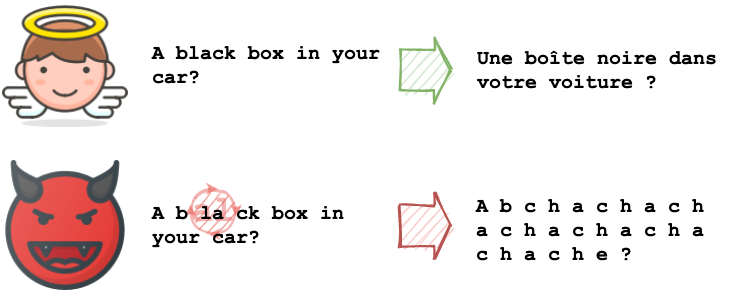
\includegraphics[scale=0.5]{figures/reordering.png}
  \caption{Homoglyfihyökkäys \citep{boucher2021bad}}
\end{figure}
\texttt{U+200F} ladotaan näkymättömänä näkymättömien merkkien tapaan.